\documentclass[letterpaper, 11pt]{article}

\usepackage{tikz, listings, comment}
\usepackage[fleqn]{amsmath}
\usepackage[margin=1in]{geometry}
\usepackage{fancyhdr, hyperref, pdfpages}
\usepackage{xcolor}

\definecolor{codegreen}{rgb}{0,0.6,0}
\definecolor{codegray}{rgb}{0.5,0.5,0.5}
\definecolor{codepurple}{rgb}{0.58,0,0.82}
\definecolor{backcolour}{rgb}{0.95,0.95,0.92}

% Disable page numbers
\pagestyle{empty}

%Basic Variables (Modify as required per homework)
\def\class{CompEn 462}
\def\homeworkNumber{2}
\def\date{02.17.2025}
\def\professor{Mark Mahon}

% Define a custom style for listings
\lstdefinestyle{mystyle}{
    backgroundcolor=\color{backcolour},   % Set background color for the code block
    commentstyle=\color{codegreen},       % Set color for comments
    keywordstyle=\color{magenta},         % Set color for keywords
    numberstyle=\tiny\color{codegray},    % Set style for line numbers
    stringstyle=\color{codepurple},       % Set color for strings
    basicstyle=\ttfamily\footnotesize,    % Set basic style for the code
    breakatwhitespace=false,              % Do not break lines at whitespace
    breaklines=true,                      % Allow breaking of lines
    captionpos=b,                         % Set caption position to bottom
    keepspaces=true,                      % Keep spaces in text
    %numbers=left,                         % Display line numbers on the left
    numbersep=5pt,                        % Set distance between line numbers and code
    showspaces=false,                     % Do not show spaces
    showstringspaces=false,               % Do not show spaces in strings
    showtabs=false,                       % Do not show tabs
    tabsize=2                             % Set tab size to 2 spaces
}

\lstset{style=mystyle}

%Code to generate new page for problem
\newcounter{problemId}
\stepcounter{problemId}
\def\newproblem{\clearpage\newpage{Problem~\arabic{problemId}\stepcounter{problemId}}\hfill\par}

%Custom Section Header Command
\newcommand{\secHeader}[1]{\vspace{2mm} \noindent \textbf{#1:}\vspace{-4mm}}

\begin{document}
%Title page
\hfill
\newline
Name: Justin Ngo
\\PSU ID: jvn5439
\\Professor: \professor
\\Class: \class
\\Date: \date

%---------------------PROBLEM 1----------------------------
\newproblem
\lstinputlisting[language = Python]{Q1 Code.py}
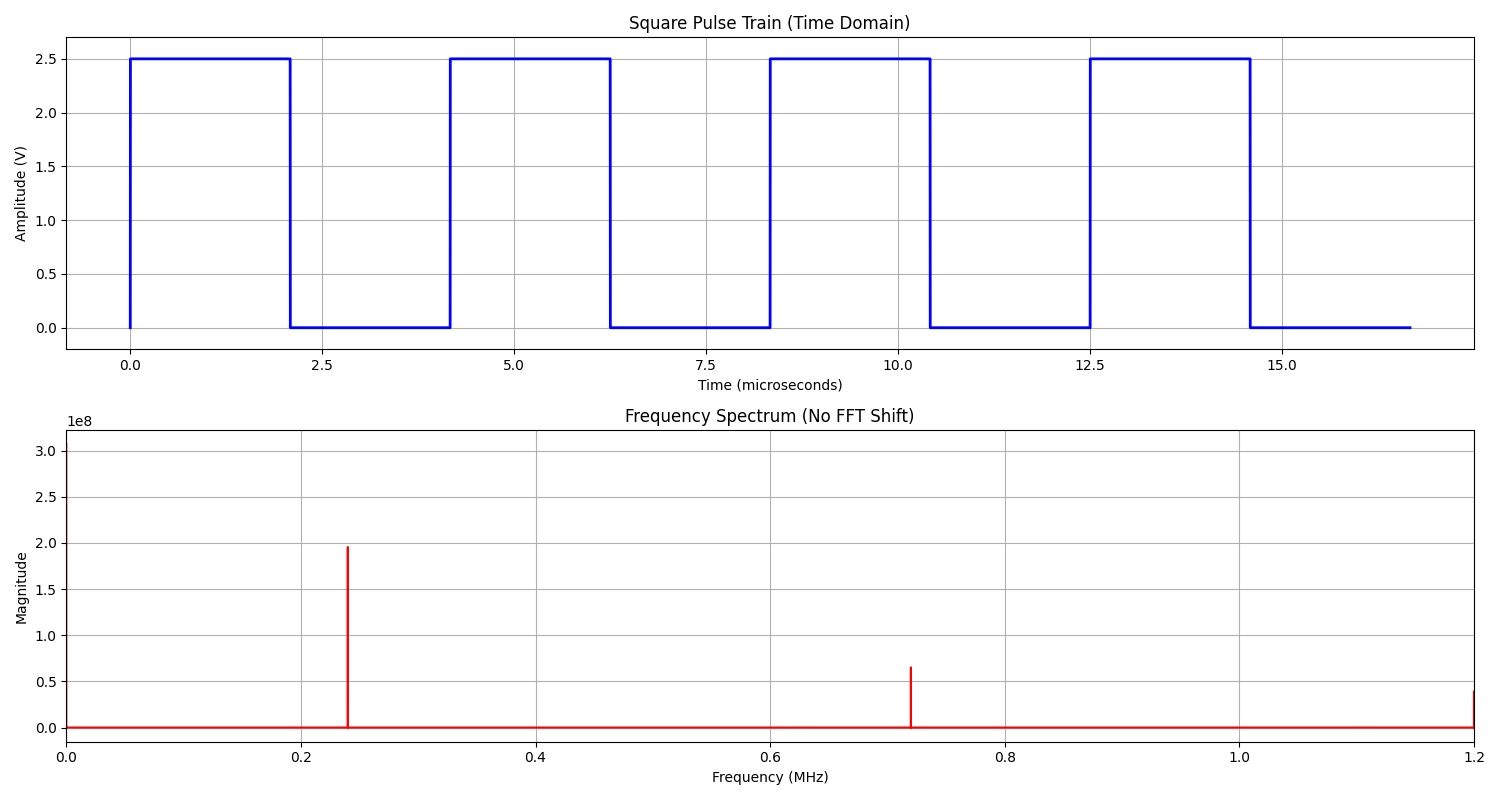
\includegraphics[width=\textwidth]{Fig1 Q1 Graphs.png}


%---------------------PROBLEM 2----------------------------
\newproblem
\lstinputlisting[language = Python]{Q2 Code.py}
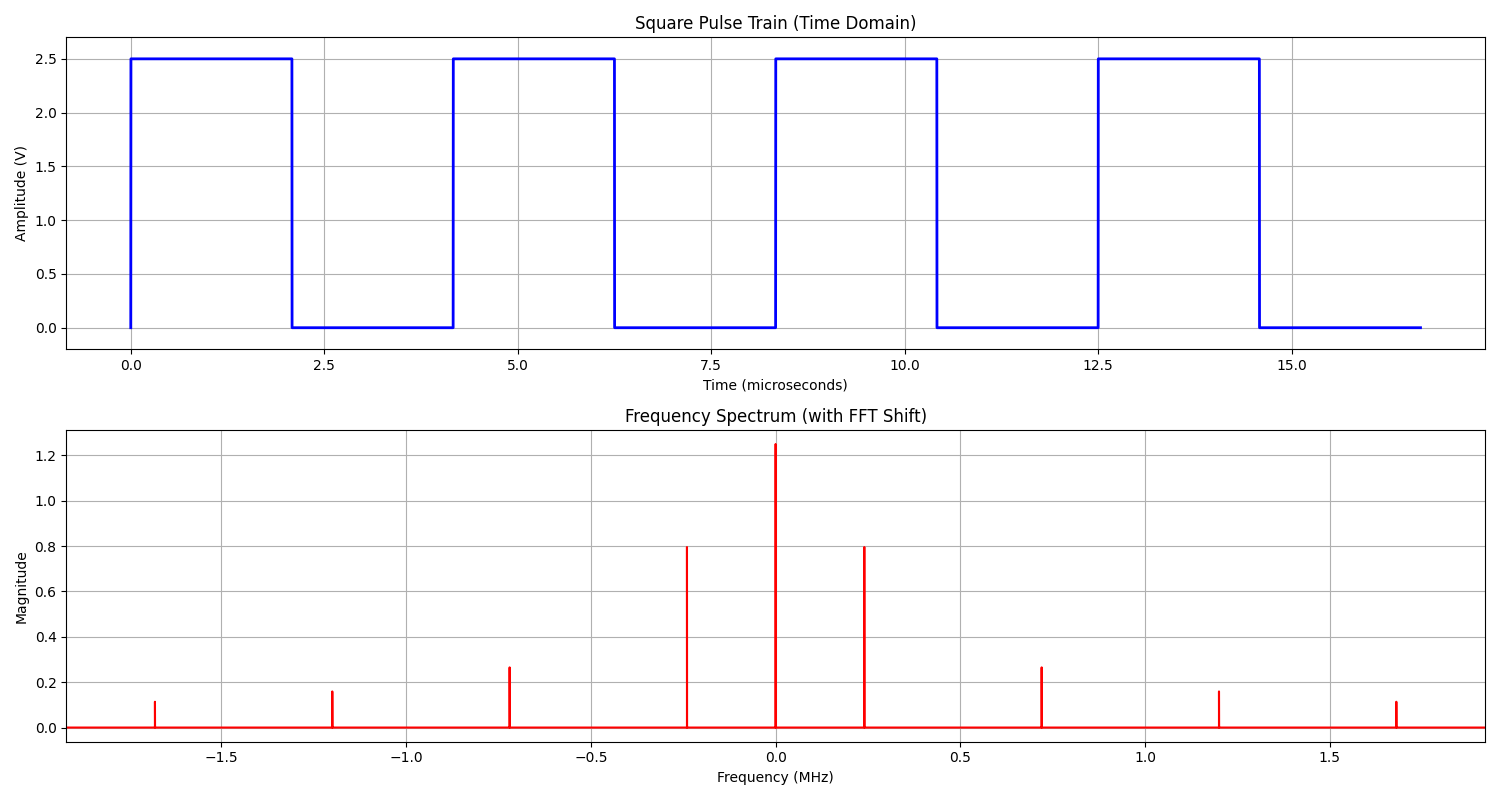
\includegraphics[width=\textwidth]{Fig2 Q2 Graphs.png}


%---------------------PROBLEM 3----------------------------
\newproblem
\secHeader{Frequencies and Amplitudes}
\vspace{10mm}

Harmonic Freqency Formula: $k \cdot $f$_o$.
\\ \indent Harmonic Amplitude Formula: $\frac{A_{max}}{k\pi}$
\begin{enumerate}
    \item DC Term (k = 0)
    \begin{enumerate}
        \item Frequency: 0
        \\$0 \cdot 240KHz = 0$
        \item Amplitude: 1.25V
        \\$\frac{2.5V}{2} = 1.25V$
    \end{enumerate}

    \item 1st Harmonic (k = 1)
    \begin{enumerate}
        \item Frequency: 240KHz
        \\$1 \cdot 240KHz = 240KHz$
        \item Amplitude: 0.8V
        \\$\frac{2.5V}{\pi} \approx 0.8V$
    \end{enumerate}

    \item 2nd Harmonic (k = 2)
    \begin{enumerate}
        \item Frequency: 480KHz
        \\$2 \cdot 240KHz = 480KHz$
        \item Amplitude: .27V
        \\$\frac{2.5V}{3\pi} \approx .27$
    \end{enumerate}

    \item 3rd Harmonic (k = 3)
    \begin{enumerate}
        \item Frequency: 720KHz
        \\$3 \cdot 240KHz = 720KHz$
        \item Amplitude: .16V
        \\$\frac{2.5V}{3\pi} \approx .16$
    \end{enumerate}

    \item 4th Harmonic (k = 4)
    \begin{enumerate}
        \item Frequency: 960KHz
        \item Amplitude: 
    \end{enumerate}
\end{enumerate}


%---------------------PROBLEM 4----------------------------
\newproblem
\lstinputlisting[language = Python]{Q3 Code.py}
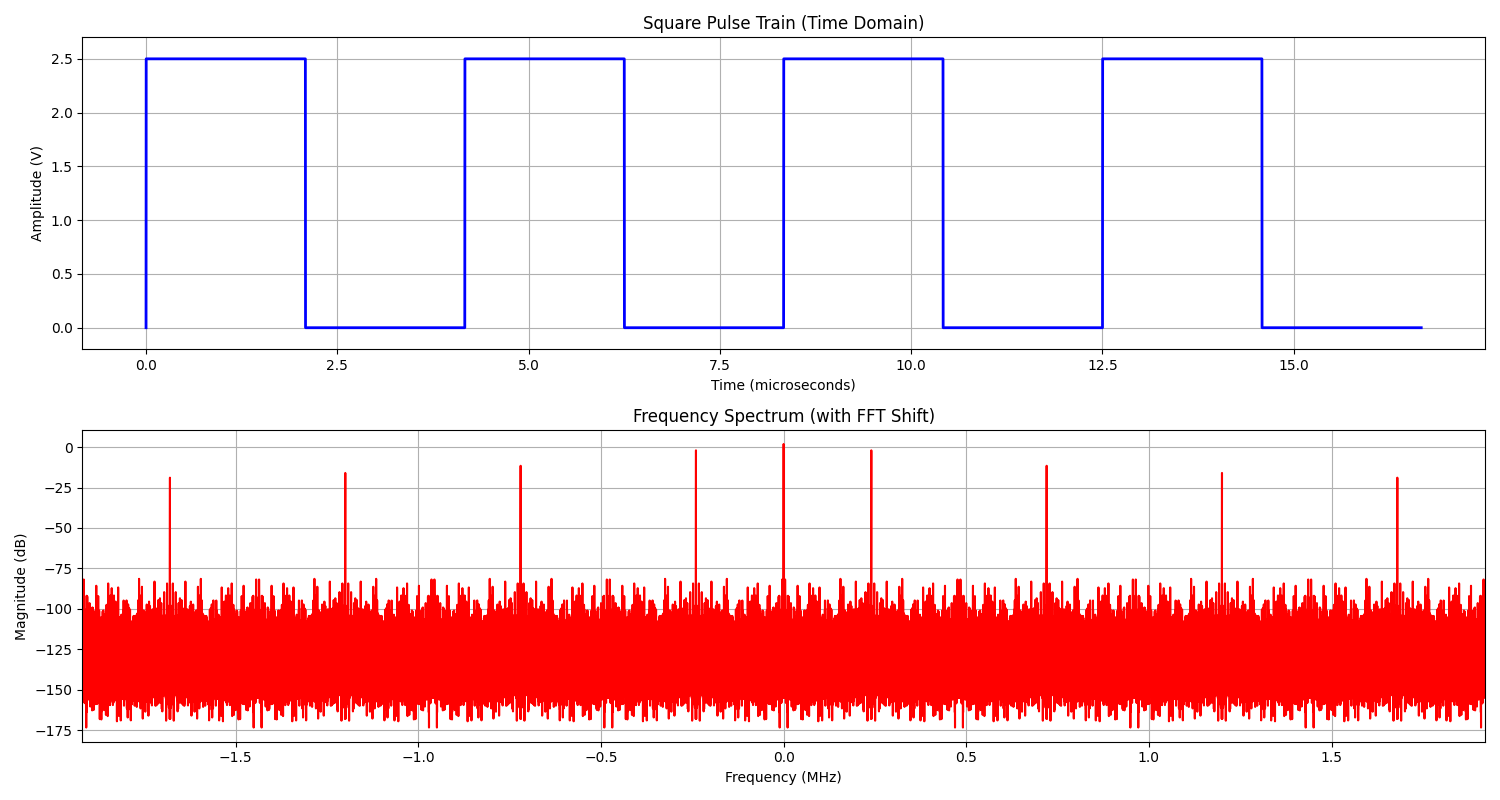
\includegraphics[width=\textwidth]{Fig3 Q3.png}

%---------------------PROBLEM 5----------------------------
\newproblem
\lstinputlisting[language = Python]{Q4 Code.py}
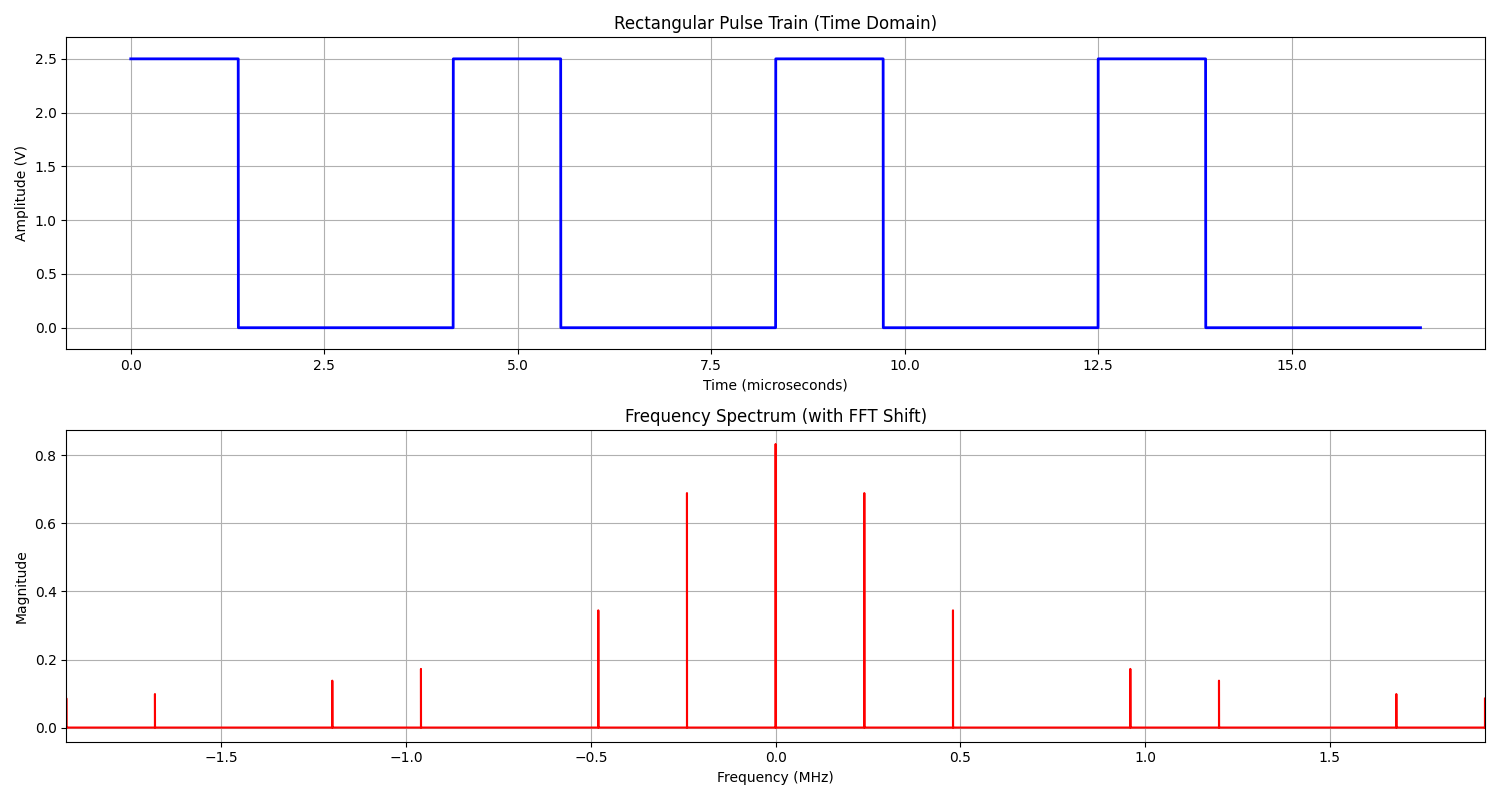
\includegraphics[width=\textwidth]{Fig4 Q4 Graphs.png}
\vspace{10mm}

The main difference between part 2 and part 4's time graphs are that the active state in part 4 is shorter than in part 2. The difference between their frequency graphs is that
the magnitudes of the later harmonics are higher, and the freqencies are more condensed and closer together.

\end{document}